\documentclass[12pt,a4paper]{article}
\usepackage[utf8]{inputenc}
\usepackage[shortlabels]{enumitem}
%Set page layout parameters
\usepackage[
top=4cm,
bottom=2cm,
left=2cm,
right=2cm,
headheight=2cm,
footskip=1cm,
marginparwidth=2cm]{geometry}
\usepackage{amsmath}
\usepackage{hyperref}
\usepackage[dvipsnames]{xcolor}
% To use color boxes
\usepackage{tcolorbox}
\usepackage{multicol}
\usepackage{lipsum}
\tcbuselibrary{listings,theorems,skins,vignette,raster,breakable,magazine,poster,fitting,hooks}
\newcounter{ejemplo}
%Images path
\graphicspath{{images/}}
\usepackage{float} %provide us with the option H
\usepackage{fancyhdr}
\usepackage{tikz}
\usepackage{tikzpagenodes}
%to redefine figure caption 
\renewcommand{\figurename}{Figura}
\renewcommand{\tablename}{Tabla}
%change text font
\usepackage[T1]{fontenc}
\usepackage{tgtermes} % LaTeX will use the TEX Gyre Bonum font family
%\usepackage{kvsetkeys}
\hypersetup{colorlinks=true,linkcolor=blue,filecolor=magenta,urlcolor=cyan}
\urlstyle{same}

\usepackage{multirow}
\usepackage{nicematrix}
\usepackage[export]{adjustbox}
\usepackage{listings}
\lstset{frame=tb,
	language=C++,
	aboveskip=3mm,
	belowskip=3mm,
	showstringspaces=false,
	columns=flexible,
	basicstyle={\small\ttfamily},
	numbers=none,
	numberstyle=\tiny\color{gray},
	keywordstyle=\color{blue},
	commentstyle=\color{dkgreen},
	stringstyle=\color{mauve},
	breaklines=true,
	breakatwhitespace=true,
	tabsize=3
}

\definecolor{subtitle_yellow}{RGB}{252,213,129}
\definecolor{title_yellow}{RGB}{249,175,16}
\definecolor{steel_blue_title}{RGB}{93,138,168}
\definecolor{pewter_blue_subtitle}{RGB}{149,178,198}
\definecolor{ecru_circle}{RGB}{215,190,130}
\definecolor{ecru_circle1}{RGB}{68,148,173}
\definecolor{dkgreen}{rgb}{0,0.6,0}
\definecolor{gray}{rgb}{0.5,0.5,0.5}
\definecolor{mauve}{rgb}{0.58,0,0.82}
\usepackage{caption}
\newcommand{\myfirststyle}{%
	\begin{tikzpicture}[remember picture, overlay]
		
		%top border
		\fill[fill=steel_blue_title](current page.north west) rectangle ([yshift=-15mm]current page.north east);
		
		\fill[fill=pewter_blue_subtitle]([yshift=-17mm]current page.north west) rectangle ([yshift=-30mm]current page.north east);
		
		%page box
		%\draw[lightgray, fill=Rhodamine, fill opacity=0.05, line width=1mm, rounded corners=3mm] ([xshift=-5mm,yshift=5mm]current page text area.north west) rectangle ([xshift=5mm,yshift=-5mm]current page text area.south east);
		
		%bottom box
		\fill[fill=pewter_blue_subtitle](current page.south west) rectangle ([yshift=10mm]current page.south east);
		
		%page circle
		\draw[white,fill=ecru_circle1,line width=2mm] ([xshift=-5mm,yshift=25mm]current page text area.north east) circle (1); 
		
		
		%page number text        
		%\node[anchor=center] at ([xshift=-5mm,yshift=25mm]current page text area.north east) {\Huge\bfseries\sffamily\color{white}{\thepage}};
		
		%title text
		\node[anchor=west] at ([yshift=32mm]current page text area.north west) {\Huge\bfseries\sffamily\color{white}{INA219 y Arduino}};
		
		%subtitle text
		\node[anchor=west] at ([xshift=10mm,yshift=16mm]current page text area.north west) {\Large\bfseries\sffamily\color{white}{}};
		
		%footer text
		\node[anchor=center] at ([yshift=-15mm]current page text area.south) {\large\bfseries\sffamily\color{white}{Created by: Rodrigo Castillejos}};
		
	\end{tikzpicture}
}


%create page style
\fancypagestyle{MyFirstStyle}{%
	\fancyhf{}
	\fancyhead[C]{\myfirststyle}
	\renewcommand{\headrulewidth}{0pt}
}%

\pagestyle{MyFirstStyle}

\colorlet{colexam}{red!75!black}
\newtcolorbox[use counter=ejemplo]{myexample}{%
	empty,title={Ejemplo \thetcbcounter},attach boxed title to top left,
	boxed title style={empty,size=minimal,toprule=2pt,top=4pt,
		overlay={\draw[colexam,line width=2pt]
			([yshift=-1pt]frame.north west)--([yshift=-1pt]frame.north east);}},
	coltitle=colexam,fonttitle=\Large\bfseries,
	before=\par\medskip\noindent,parbox=false,boxsep=0pt,left=0pt,right=3mm,top=4pt,
	breakable,pad at break*=0mm,vfill before first,
	overlay unbroken={\draw[colexam,line width=1pt]
		([yshift=-1pt]title.north east)--([xshift=-0.5pt,yshift=-1pt]title.north-|frame.east)
		--([xshift=-0.5pt]frame.south east)--(frame.south west); },
	overlay first={\draw[colexam,line width=1pt]
		([yshift=-1pt]title.north east)--([xshift=-0.5pt,yshift=-1pt]title.north-|frame.east)
		--([xshift=-0.5pt]frame.south east); },
	overlay middle={\draw[colexam,line width=1pt] ([xshift=-0.5pt]frame.north east)
		--([xshift=-0.5pt]frame.south east); },
	overlay last={\draw[colexam,line width=1pt] ([xshift=-0.5pt]frame.north east)
		--([xshift=-0.5pt]frame.south east)--(frame.south west);},%
}


\begin{document}
	Los dispositivos que monitorean y reportan la corriente de un sistema pueden proporcionar ya sea una salida analógica que es proporcional a la corriente sensada, o comunicar la corriente a un procesador digitalmente. El uso de amplificadores de sensado de corriente digitales son comunmente preferidos porque la conversión analógica a digital integrada permite que los datos sean enviados directamente al controlador o procesador principal. La interacción con el procesador central requiere de una interface digital que permite tanto el envío como la recepción de instrucciones así como de datos. Para las aplicaciones de sensado de corriente las interfaces digitales más comunmente utilizadas son $I^2C$, SMBus, PMBus y SPI. \\
	
	\noindent \textbf{Descripción}\\\\
	El INA219 es un monitor de potencia compatible con las interfaces $I^{2}C$ o SMBus. El dispositivo monitorea tanto la caída de voltaje de derivación como el voltaje de bus. Un valor de calibración programable, combinado con un multiplicador interno posibilita la lectura de la corriente en ampers. Un registro multiplicador adicional calcula la potencia en watts.
	
	El INA219 está disponible en dos grados: A y B. La versión de grado B tiene mayores especificaciones de precisión. El INA219 es capaz de consumir un máximo de 1 mA de corriente y opera en el rango de -40°C a 125°C.\\
	
	\noindent \textbf{Características}
	\begin{itemize}
		\item Sensa el voltaje de bus desde 0 a 26V
		\item Reporta la corriente, voltaje y potencia
		\item 16 direcciones programables
		\item Opciones de filtrado
		\item Registros de calibración
		\item SOT23-8 y SOIC-8
	\end{itemize}

	\noindent \textbf{Configuración de pines y funciones}
	\begin{figure}[H]
		\centering
		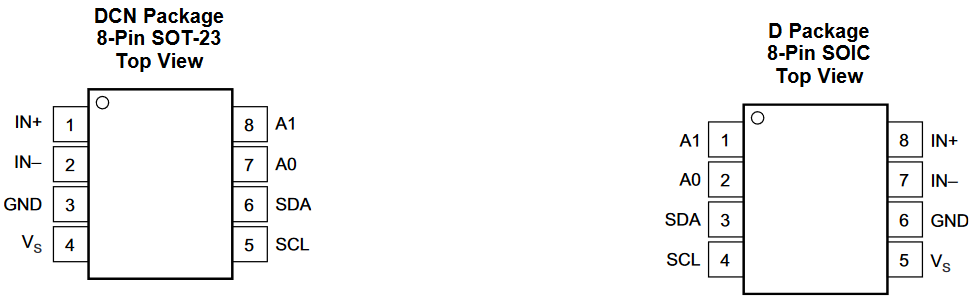
\includegraphics[scale=0.8]{packages}
		\label{fig:packages}
		\caption{Tipos de encapsulado para el INA219}
	\end{figure}
	
	\begin{figure}[H]
	\centering
	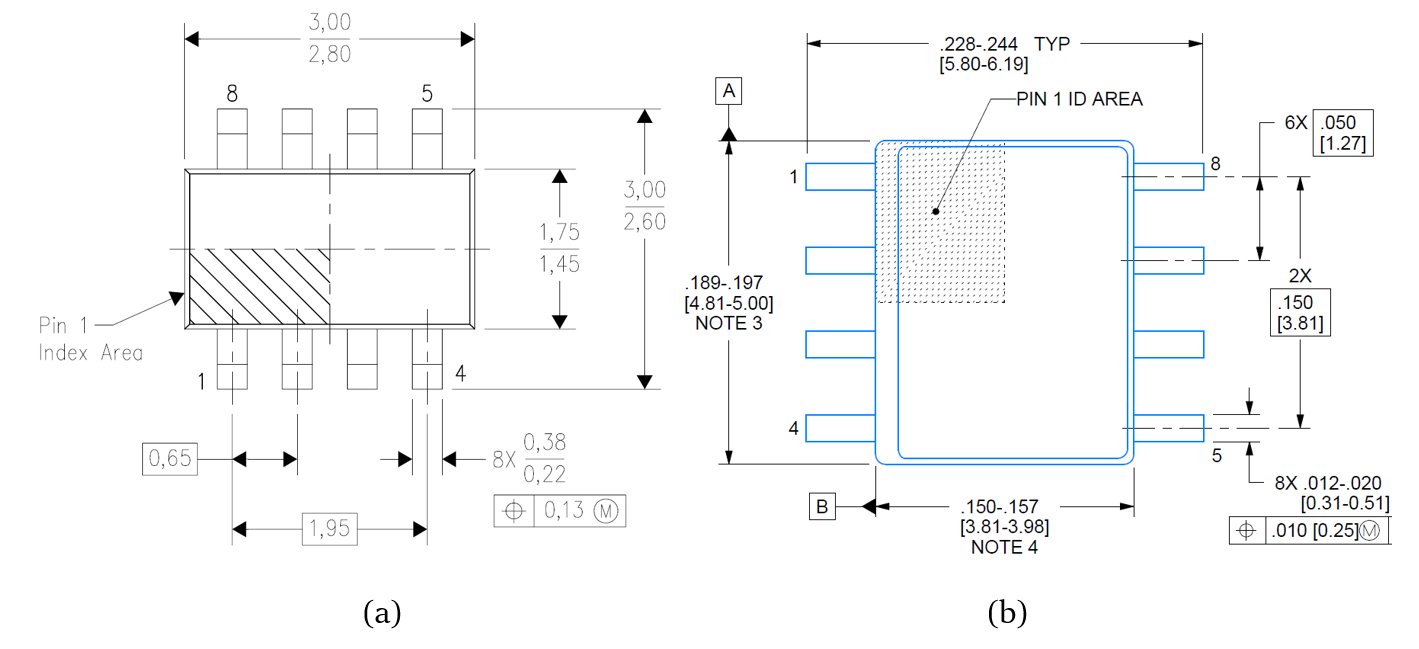
\includegraphics[scale=0.6]{packages2}
	\label{fig:packages2}
	\caption{(a) DCN Package SOT-23 and (b) D Package SOIC}
	\end{figure}

	%\Block[v-center]
	\begin{table}[H]
		\centering
	\begin{NiceTabular}{cccp{1.6	cm}p{8cm}}[hvlines]
		\Block[fill=gray!20]{1-3}{PIN} & & & \Block[fill=gray!20]{2-1}{IO} & \Block[fill=gray!20]{2-1}{DESCRIPTION} \\
		\Block[fill=gray!20]{1-1}{NAME} & \Block[fill=gray!20]{1-1}{SOT-23} & \Block[fill=gray!20]{1-1}{SOIC} \\
		\Block[c]{1-1}{\texttt{IN+}} & \verb|1| & \verb|8| & \texttt{Analog Input} & \texttt{Positive differential shunt voltage. Connect to positive side of shunt resistor}\\
		\texttt{IN-} & \verb|2| & \verb|7| & \texttt{Analog Input} & \texttt{Negative differential shunt voltage. Connect to negative side of shunt resistor. Bus voltage is measured from this pin to ground.}\\
		\texttt{GND} & \verb|3| & \verb|6| & \texttt{Analog} & \texttt{Ground}\\
		\texttt{Vs} & \verb|4| & \verb|5| & \texttt{Analog} & \texttt{Power supply, 3 to 5.5V}\\
		\texttt{SCL} & \verb|5| & \verb|4| & \texttt{Digital Input} & \texttt{Serial bus clock line}\\
		\texttt{SDA} & \verb|6| & \verb|3| & \texttt{Digital I/O} & \texttt{Serial bus data line}\\
		\texttt{A0} & \verb|7| & \verb|2| & \texttt{Digital Input} & \texttt{Address pin}\\
		\texttt{A1} & \verb|8| & \verb|1| & \texttt{Digital Input} & \texttt{Address pin}\\		
	\end{NiceTabular}
	\caption{Configuración de pines}
	\label{tab:table1}
	\end{table}

	\newpage
	%\vspace{0.5cm}
	\noindent \textbf{Descripción detallada}\\\\
	El INA219 es un amplificador de sensado de corriente digital compatible con interface $I^2C$ y SMBus. Proporciona lecturas de voltaje, corriente y potencia. Los registros programables permiten además una configuración flexible en la resolución de las mediciones así como operación continua contra una operación de disparo.\\
	
	\noindent \textbf{Configuración básica del ADC}\\\\
	Las dos entradas analógicas del \texttt{INA219}, \texttt{IN+} e \texttt{IN-}, se conectan a un resistor de derivación en el bus de interés. El \texttt{INA219} se alimenta típicamente con una fuente de alimentación separada desde $3$ a $5.5\,V$. El bus a ser sensado puede variar de entre $0$ a $26\,V$. No existe ninguna consideración especial en la secuencia de alimentación (por ejemplo, puede estar prersente un voltaje de bus mientras que la alimentación del dispositivo está en \texttt{off}, y viceversa).
	
	El \texttt{INA219} sensa la pequeña caída de voltaje en el resistor de derivación para obtener el voltaje de derivación y sensa el voltaje con respecto a tierra desde \texttt{IN-} para obtener el voltaje de bus. La figura \ref{fig:ina219_diagram} muestra esta operación.\\

	\begin{figure}[H]
		\centering
		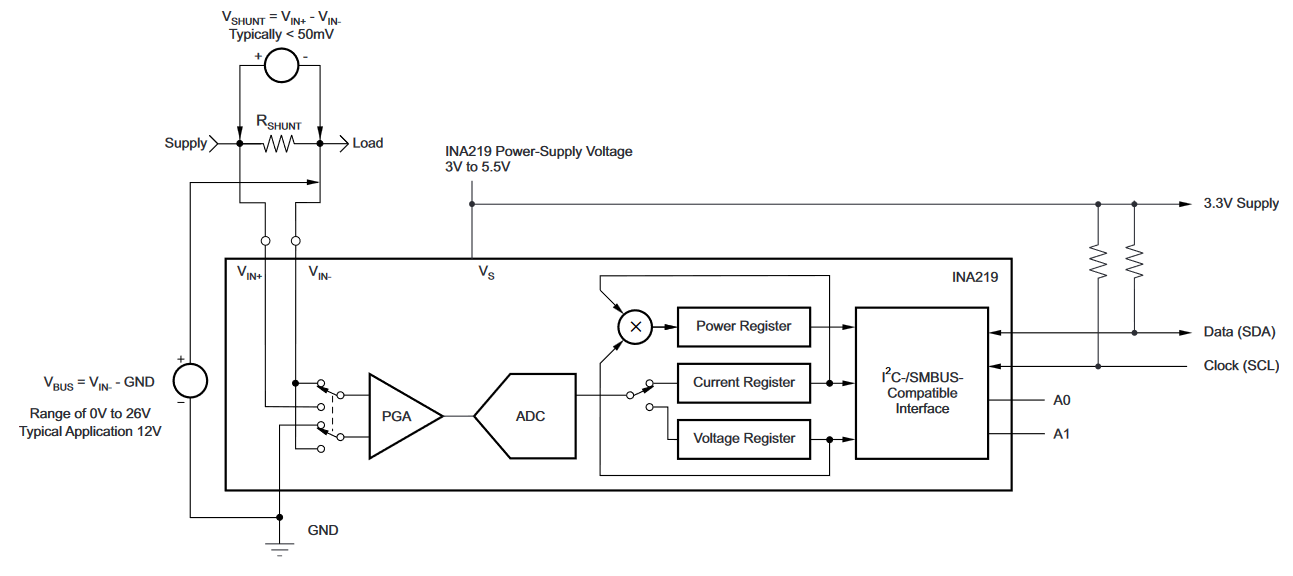
\includegraphics[scale=0.6]{diagram}
		\caption{INA219 configurado para medir el voltaje de derivación y de bus}
		\label{fig:ina219_diagram}
	\end{figure}

	A pesar de que el \texttt{INA219} puede realizar una lectura de sus valores a cualquier hora, y el dato desde la última conversión permanece disponible, el bit de conversión lista (Registro de Voltaje de Bus, bit CNVR) puede ayudar a coordinar conversiones del tipo one-sjout o de disparo. El bit de conversión lista se establece una vez que todas las conversiones, operaciones de promediado y multiplicación estén completas.\\
	
	\noindent \textbf{Programabilidad}\\
	Después de programar el Registro de Calibración, el registro de corriente \texttt{Current Register (04h)} y el Registro de Potencia \texttt{Power Register (03h)} se actualizan basados en las correspondientes mediciones del voltaje de derivación y voltaje de bus. Hasta que el Registro de Calibración sea programado, los Registros de Corriente y Potencia permanecen en cero.
	
	\begin{tcolorbox}[colback=red!10!white,colframe=red!50!black,title=Nota]
		Después de programar el Registro de Calibración (\texttt{Calibration Register}), el \texttt{Current Register (04h)} y el \texttt{Power Register (03h)} se actualizan basados en las mediciones correspondientes del voltaje de derivación y del voltaje de bus. Hasta que el \texttt{Calibration Register} es programado, el \texttt{Current Register (04h)} y el \texttt{Power Register (03h)} permanecen en cero.
	\end{tcolorbox}

	\noindent \textbf{Programación del Registro de Calibración}\\\\
	La programación del Registro de Calibración se basa en la ecuación 1. Esta ecuación incluye el término \texttt{Current\_LSB}, el cual es el valor programado para el bit menos significativo (LSB) del Registro de Corriente (\texttt{04h})
	
	\begin{tcolorbox}[colback=red!5!white,colframe=red!75!black,width=(\linewidth+0.45cm)]
		\begin{equation}
				\verb|Cal| = \verb|trunc|\left( \frac{0.04096}{\texttt{Current\_LSB}\times R_{SHUNT}} \right)
		\end{equation}
	\end{tcolorbox}

	Donde:
	\begin{align}
		\texttt{Current\_LSB} &= \frac{\texttt{Maximum Expected Current}}{2^{15}}\\
		\texttt{Power\_LSB} &= 20 \times \texttt{Current\_LSB}
	\end{align}

	\begin{tcolorbox}[colback=cyan!10!white,colframe=cyan!50!black,title=Voltaje de Derivación]
		El voltaje de Derivación se calcula multiplicando el contenido del Registro del Voltaje de Derivación por $10 \mu V$ 
	\end{tcolorbox}
	
	\begin{tcolorbox}[colback=cyan!10!white,colframe=cyan!50!black,title=Voltaje de Bus]
		Los bits del Registro de Voltaje de Bus no están alineados a la derecha. Con el fin de calcular el valor del Voltaje de Bus, el contenido del Registro de Voltaje de Bus debe ser \textbf{desplazado a la derecha} por \textbf{tres bits}. Posteriormente el contenido debe ser multiplicado por $4 \, mV$ para calcular el voltaje de bus medido por el dispositivo
	\end{tcolorbox}
	
	\begin{tcolorbox}[colback=cyan!10!white,colframe=cyan!50!black,title=Valor de la corriente]
		Para obtener el valor de la corriente en amperes, el registro de Corriente debe ser multiplicado por el valor programado de \texttt{Current\_LSB}
	\end{tcolorbox}

	\begin{tcolorbox}[colback=cyan!10!white,colframe=cyan!50!black,title=Valor de la potencia]
		Para obtener el valor de la potencia en watts, el registro de Potencia debe ser multiplicado por el valor programado de \texttt{Power\_LSB} el cual es 20 veces el valor de \texttt{Current\_LSB}.
	\end{tcolorbox}

	\vspace{0.3cm}
	Después de programar el Registro de Calibración, el valor esperado en el Registro de Corriente \texttt{04h} puede calcular multiplicando el contenido del Registro de Voltaje de Derivación por el Registro de Calibración y entonces dividirlo por \texttt{4096} como se muestra en la ecuación 4.
	
	\begin{align}
		\texttt{Current Register} = \frac{\texttt{Shunt Voltage Register} \times \texttt{Calibration Register}}{4096}
	\end{align}

	El valor esperado en el Registro de Potencia \texttt{(03h)} puede calcularse multiplicando el valor del Registro de Corriente por el valor del Registro de Voltaje de Bus y entonces dividirlo entre 5000 como se muestra en la ecuación 5. 
	
	\begin{align}
		\texttt{Power Register} = \frac{\texttt{Current Register} \times \texttt{Bus Voltage Register}}{5000}
	\end{align}

	 \begin{tcolorbox}[colback=red!10!white,colframe=red!50!black,title=Configuaciones por defecto. Sin necesidad de programar]
	 	el \texttt{INA219} puede ser usado sin necesidad de programarlo y si sólo es necesario leer la caída de voltaje de derivación y el voltaje de bus con una resolución por defecto de 12 bits, un rango de escala completa de derivación de 320mV (PGA = /8), un ango de bus de escala completa de 32V y una conversión continua de voltaje de deivación y de bus.
	 \end{tcolorbox}
 
 	\vspace{0.3cm}
 	\noindent \textbf{Direcciones del bus serial}\\\\
 	Para comunicarse con el \texttt{INA219}, el maestro debe primero direccionar el dispositivo a través del byte de dirección del esclavo, el cual consiste de una dirección de 7 bits.
 	El \texttt{INA219} cuanta con dos pines de dirección, \texttt{A0} y \texttt{A1}. La tabla \ref{tab:table2} muestra los niveles lógicos de los pines para cada una de las 16 direcciones posibles.
 	
 	\begin{table}[H]
 		\centering
 	 \begin{NiceTabular}{ccc}[hvlines]
 	 	\Block[fill=gray!20]{1-1}{A1} & \Block[fill=gray!20]{1-1}{A0} & \Block[fill=gray!20]{1-1}{SLAVE ADDRESS} \\
 	 	GND & GND & \texttt{1000000}\\
 	 	GND & $V_{S+}$ & \texttt{1000001}\\
 	 	GND & SDA &  \texttt{1000010}\\
 	 	GND & SCL & \texttt{1000011}\\
 	 	$V_{S+}$ & GND & \texttt{1000100}\\
 	 	$V_{S+}$ & $V_{S+}$ & \texttt{1000101}\\
 	 	$V_{S+}$ & SDA & \texttt{1000110}\\
 	 	$V_{S+}$ & SCL & \texttt{1000111}\\
 	 	SDA & GND & \texttt{1001000}\\
 	 	SDA & $V_{S+}$ & \texttt{1001001}\\
 	 	SDA & SDA & \texttt{1001010}\\
 	 	SDA & SCL & \texttt{1001011}\\
 	 	SCL & GND & \texttt{1001100}\\
 	 	SCL & $V_{S+}$ & \texttt{1001101}\\
 	 	SCL & SDA & \texttt{1001110}\\
 	 	SCL & SCL & \texttt{1111111}\\
 	 \end{NiceTabular}
  \caption{Configuración de pines}
  \label{tab:table2}
  	\end{table}
  
  %\vspace{0.3cm}
  \newpage
  \noindent \textbf{Mapa de Registros}\\\\
  El \texttt{INA219} usa un banco de registros para almacenar los ajustes de configuración, resultados de medición, límites máximos y mínimos e información de estado. La tabla \ref{tab_table3} resume los registros del \texttt{INA219}
  
  %row-column
  \begin{table}[H]
  	\fontsize{7pt}{12pt}\selectfont
  \begin{NiceTabular}{p{2cm}p{2.6cm}p{5cm}p{3cm}cc}[hvlines]
  	\Block[fill=gray!20,v-center]{1-1}{POINTER ADDR} & \Block[fill=gray!20]{2-1}{REGISTER NAME} & \Block[fill=gray!20]{2-1}{FUNCTION} & \Block[fill=gray!20,v-center]{1-2}{POWER-ON RESET} & & \Block[fill=gray!20]{2-1}{TYPE}\\
  	\Block[fill=gray!20]{1-1}{HEX} & & & \Block[fill=gray!20]{1-1}{BINARY} & \Block[fill=gray!20]{1-1}{HEX} &  \\
  	\Block[v-center]{1-1}{\texttt{00}} & \Block[v-center]{1-1}{Configuration} & All-Register reset, settings for bus voltage range, PGA Gain, ADC resolution/averaging & \Block[v-center]{1-1}{\texttt{00111001 10011111}} & \Block[v-center]{1-1}{\texttt{399F}} & \Block[v-center]{1-1}{R/W}\\
  	\Block[v-center]{1-1}{\texttt{01}} & \Block[v-center]{1-1}{Shunt Voltage} & Shunt Voltage measurement data & \Block[v-center]{1-1}{Shunt Voltage} & - & \Block[v-center]{1-1}{R}\\
  	\Block[v-center]{1-1}{\texttt{02}} & \Block[v-center]{1-1}{Bus Voltage} & Bus Voltage measurement data & \Block[v-center]{1-1}{Bus Voltage} & - & \Block[v-center]{1-1}{R}\\
  	\Block[v-center]{1-1}{\texttt{03}} & \Block[v-center]{1-1}{Power} & Power measurement data & \Block[v-center]{1-1}{\texttt{00000000 00000000}} & \Block[v-center]{1-1}{\texttt{0000}} & \Block[v-center]{1-1}{R}\\
  	\Block[v-center]{1-1}{\texttt{04}} & \Block[v-center]{1-1}{Current} & Contains the value of the current flowing through the shunt resistor & \Block[v-center]{1-1}{\texttt{00000000 00000000}} & \Block[v-center]{1-1}{\texttt{0000}} & \Block[v-center]{1-1}{R}\\
  	\Block[v-center]{1-1}{\texttt{05}} & \Block[v-center]{1-1}{Calibration} & Sets the full scale range and LSB of the current and power measurements. Overall system calibration & \Block[v-center]{1-1}{\texttt{00000000 00000000}} & \Block[v-center]{1-1}{\texttt{0000}} & \Block[v-center]{1-1}{R/W}
  \end{NiceTabular}
	\caption{Registros del INA219}
	\label{tab_table3}
	\end{table}

	\begin{myexample}
	\noindent \textbf{Requerimientos de diseño. Programación del 1NA219}\\\\
	El \texttt{INA219} mide el voltaje  através de una resistencia de sensado de corriente $(R_{SHUNT})$ cuando la corriente pasa a través del resistor. El dispositivo también mide el voltaje de bus y calcula la potencia una vez que está calibrado.
	
	\noindent Las condiciones para el circuito de ejemplo son: corriente máxima 500mA, corriente nominal: 100mA, $V_{CM} = 5V$, $R_{SHUNT}$ $= 100m\Omega$, $V_{SHUNT}FSR = (100m\Omega)(500mA) = 50mV (PGA /2 = 80mV)$ (no obstante utilizaremos el valor de PGA/1 = 40mV ya que no se alcanzará el valor de la corriente máxima) y $BRGN = 0$ (rango de VBUS = 16 V)
	
	Usamos la ecuación 2 para calcular el valor de \texttt{Current\_LSB}
	\begin{align}
		\texttt{Current\_LSB} = \frac{\texttt{Maximun Expected Current}}{2^{15}} = \frac{500\,mA}{2^{15}} = 15.30 \frac{\mu A}{bit}\nonumber
	\end{align}

	Ahora usamos la ecuación 1 para encontrar el valor de $Cal$. Este valor es el que será programado en el registro de calibración.
	\begin{equation}
		\verb|Cal| = \verb|trunc|\left( \frac{0.04096}{\texttt{Current\_LSB}\times R_{SHUNT}} \right) = \texttt{truc} \left( \frac{0.04096}{(15.30 \mu A)(100 m\Omega)} \right) = 26772 \nonumber
	\end{equation}
	
	El siguiente paso es escribir los bits necesarios en el Registro de Configuración (0x00)
	\begin{figure}[H]
		\centering
		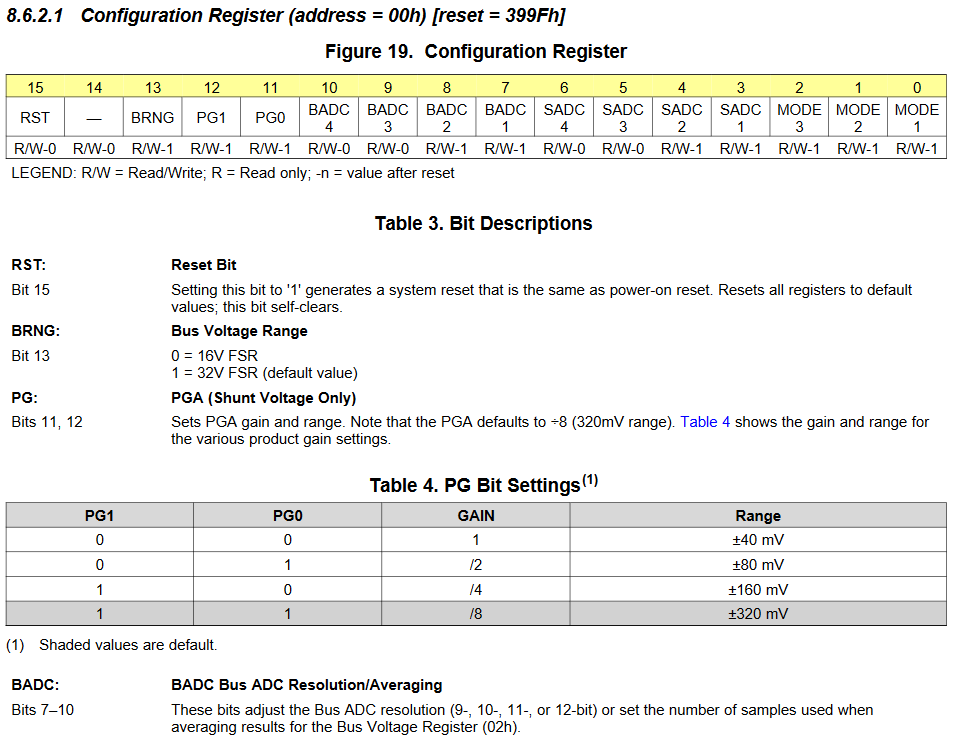
\includegraphics[scale=0.63]{configuration_register1}
		\label{fig:configuration_register1}
	\end{figure}
\begin{figure}[H]
	\centering
	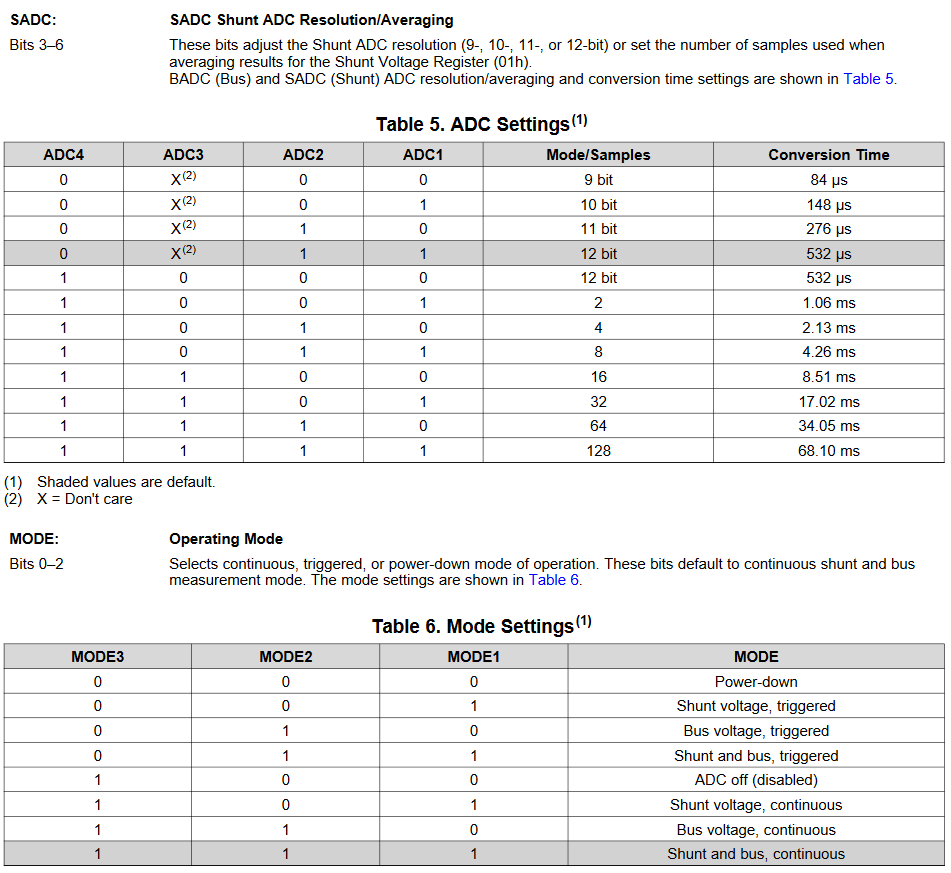
\includegraphics[scale=0.63]{configuration_register2}
	\label{fig:configuration_register2}
\end{figure}

	Establecemos los siguientes bits del registro:
	\begin{table}[H]
		\fontsize{6pt}{10pt}\selectfont
		\centering
		\begin{NiceTabular}{cccccccccccccccc}[hvlines]
			\Block[v-center]{1-1}{15} & \Block[v-center]{1-1}{14} & \Block[v-center]{1-1}{13} & \Block[v-center]{1-1}{12} & \Block[v-center]{1-1}{11} & \Block[v-center]{1-1}{10} & \Block[v-center]{1-1}{9} & \Block[v-center]{1-1}{8} & \Block[v-center]{1-1}{7} & \Block[v-center]{1-1}{6} & \Block[v-center]{1-1}{5} & \Block[v-center]{1-1}{4} & \Block[v-center]{1-1}{3} & \Block[v-center]{1-1}{2} & \Block[v-center]{1-1}{1} & \Block[v-center]{1-1}{0} \\
			\Block[v-center]{1-1}{RST} & - & BRGN & PG1 & PG0 & BADC4 & BADC3 & BADC2 & BADC1 & SADC4 & SADC3 & SADC2 & SADC1  & MODE3 & MODE2 & MODE1 \\
			\Block[v-center]{1-1}{0} & 0 & 0 & 0 & 0 & 0 & 0 & 1 & 1 & 0 & 0 & 1 & 1 & 1 & 1 & 1 \\
		\end{NiceTabular}
	\end{table}
	Esta combinación de bits es el equivalente a $415_{10}$ o $019F_{16}$ en el Registro de configuración
	
	\end{myexample}
	\begin{lstlisting}
		#include <Arduino.h>
		#include <Wire.h>
		#include <math.h>
		#define INA219_ADDRESS 0X40          
		#define CONFIG_REGISTER 0X00           
		#define SHUNT_VOLTAGE_REGISTER 0X01   
		#define BUS_VOLTAGE_REGISTER 0X02     
		#define POWER_REGISTER 0X03           
		#define CURRENT_REGISTER 0X04        
		#define CALIBRATION_REGISTER 0X05  
		
		uint16_t calibration_value = 26842; 
		uint16_t config_value = 415; //00000 0001 1001 1111
		uint16_t calibration_result;
		uint16_t config_result;
		uint16_t shunt_volt_content;
		uint16_t bus_volt_content;
		uint16_t current_content;
		uint16_t power_content;
		byte calibration_high_byte;
		byte calibration_low_byte;
		byte config_high_byte;
		byte config_low_byte;
		byte shunt_volt_high_byte;
		byte shunt_volt_low_byte;
		byte bus_volt_high_byte;
		byte bus_volt_low_byte;
		byte current_high_byte;
		byte current_low_byte;
		byte power_high_byte;
		byte power_low_byte;
		float shunt_volt_result;
		float bus_volt_result;
		float current_result;
		float power_result;
		float max_current = 0.5;
		float current_LSB = max_current / (pow (2, 15));
		float power_LSB = 20 * current_LSB;
		
		void setup() {
			Serial.begin(9600);
			
			//Writing the value of calibration_value in CALIBRATION register
			Wire.begin();
			Wire.beginTransmission(INA219_ADDRESS);
			Wire.write(CALIBRATION_REGISTER);
			Wire.write(highByte(calibration_value));
			Wire.write(lowByte(calibration_value));
			Wire.endTransmission();
			delay(100);
			
			//Writing the value of config_value in CONFIGURATION register
			Wire.beginTransmission(INA219_ADDRESS);
			Wire.write(CONFIG_REGISTER);
			Wire.write(highByte(config_value));
			Wire.write(lowByte(config_value));
			Wire.endTransmission();
			delay(100);
			
			//Reading calibration and configuration registers to ensure the data is correct
			Wire.beginTransmission(INA219_ADDRESS);
			Wire.write(CALIBRATION_REGISTER);
			Wire.endTransmission(); 
			Wire.requestFrom(INA219_ADDRESS, 2);
			calibration_high_byte = Wire.read();
			calibration_low_byte = Wire.read();
			calibration_result = ((calibration_high_byte << 8) | calibration_low_byte);
			
			delay(100);
			
			Wire.beginTransmission(INA219_ADDRESS);
			Wire.write(CONFIG_REGISTER);
			Wire.endTransmission();
			Wire.requestFrom(INA219_ADDRESS, 2);
			config_high_byte = Wire.read();
			config_low_byte = Wire.read();
			config_result = ((config_high_byte << 8) | config_low_byte);
			
			delay(100);
			Serial.println();
			
			Serial.print("calibration register result: ");
			Serial.println(calibration_result, DEC);
			Serial.print("configuration register result: ");
			Serial.println(config_result, DEC);
		}
		
		void loop() {
			//Reading SHUNT VOLTAGE register
			Wire.beginTransmission(INA219_ADDRESS);
			Wire.write(SHUNT_VOLTAGE_REGISTER);
			Wire.endTransmission();
			Wire.requestFrom(INA219_ADDRESS, 2);
			shunt_volt_high_byte = Wire.read();
			shunt_volt_low_byte = Wire.read();
			shunt_volt_content = ((shunt_volt_high_byte << 8) | shunt_volt_low_byte);
			//Serial.print(shunt_volt_content, DEC);
			shunt_volt_result = (float)shunt_volt_content * (10.0/1000000.0) * (1000); // result is multipied by 1000 to express the value in mV
			
			delay(100);
			//Reading BUS VOLTAGE register
			Wire.beginTransmission(INA219_ADDRESS);
			Wire.write(BUS_VOLTAGE_REGISTER);
			Wire.endTransmission();
			Wire.requestFrom(INA219_ADDRESS, 2);
			bus_volt_high_byte = Wire.read();
			bus_volt_low_byte = Wire.read();
			bus_volt_content = (((bus_volt_high_byte << 8) | bus_volt_low_byte)) >> 3;
			bus_volt_result = (float)bus_volt_content * (4.0 / 1000.0); 
			
			delay(100);
			//Reading CURRENT register
			Wire.beginTransmission(INA219_ADDRESS);
			Wire.write(CURRENT_REGISTER);
			Wire.endTransmission();
			Wire.requestFrom(INA219_ADDRESS, 2);
			current_high_byte = Wire.read();
			current_low_byte = Wire.read();
			current_content = ((current_high_byte << 8) | current_low_byte);
			current_result = (float)current_content * current_LSB * 1000.0; // is multiplied by 100 to express the result in mA
			
			delay(100);
			//Reading POWER register
			Wire.beginTransmission(INA219_ADDRESS);
			Wire.write(POWER_REGISTER);
			Wire.endTransmission();
			Wire.requestFrom(INA219_ADDRESS, 2);
			power_high_byte = Wire.read();
			power_low_byte = Wire.read();
			power_content = ((power_high_byte << 8) | power_low_byte);
			power_result = (float)power_content * power_LSB * 1000.0; // is multiplied by 100 to express the result in mW
			
			Serial.print("Shunt voltage register result: ");
			Serial.print(shunt_volt_result, DEC);
			Serial.println(" mV");
			Serial.print("Bus voltage register result: ");
			Serial.print(bus_volt_result, DEC);
			Serial.println(" V");
			Serial.print("Current result: ");
			Serial.print(current_result);
			Serial.println(" mA");
			Serial.print("Power result: ");
			Serial.print(power_result);
			Serial.println(" mW");
			delay(5000);
			
		}
	\end{lstlisting}
	
	\begin{figure}[H]
		\centering
		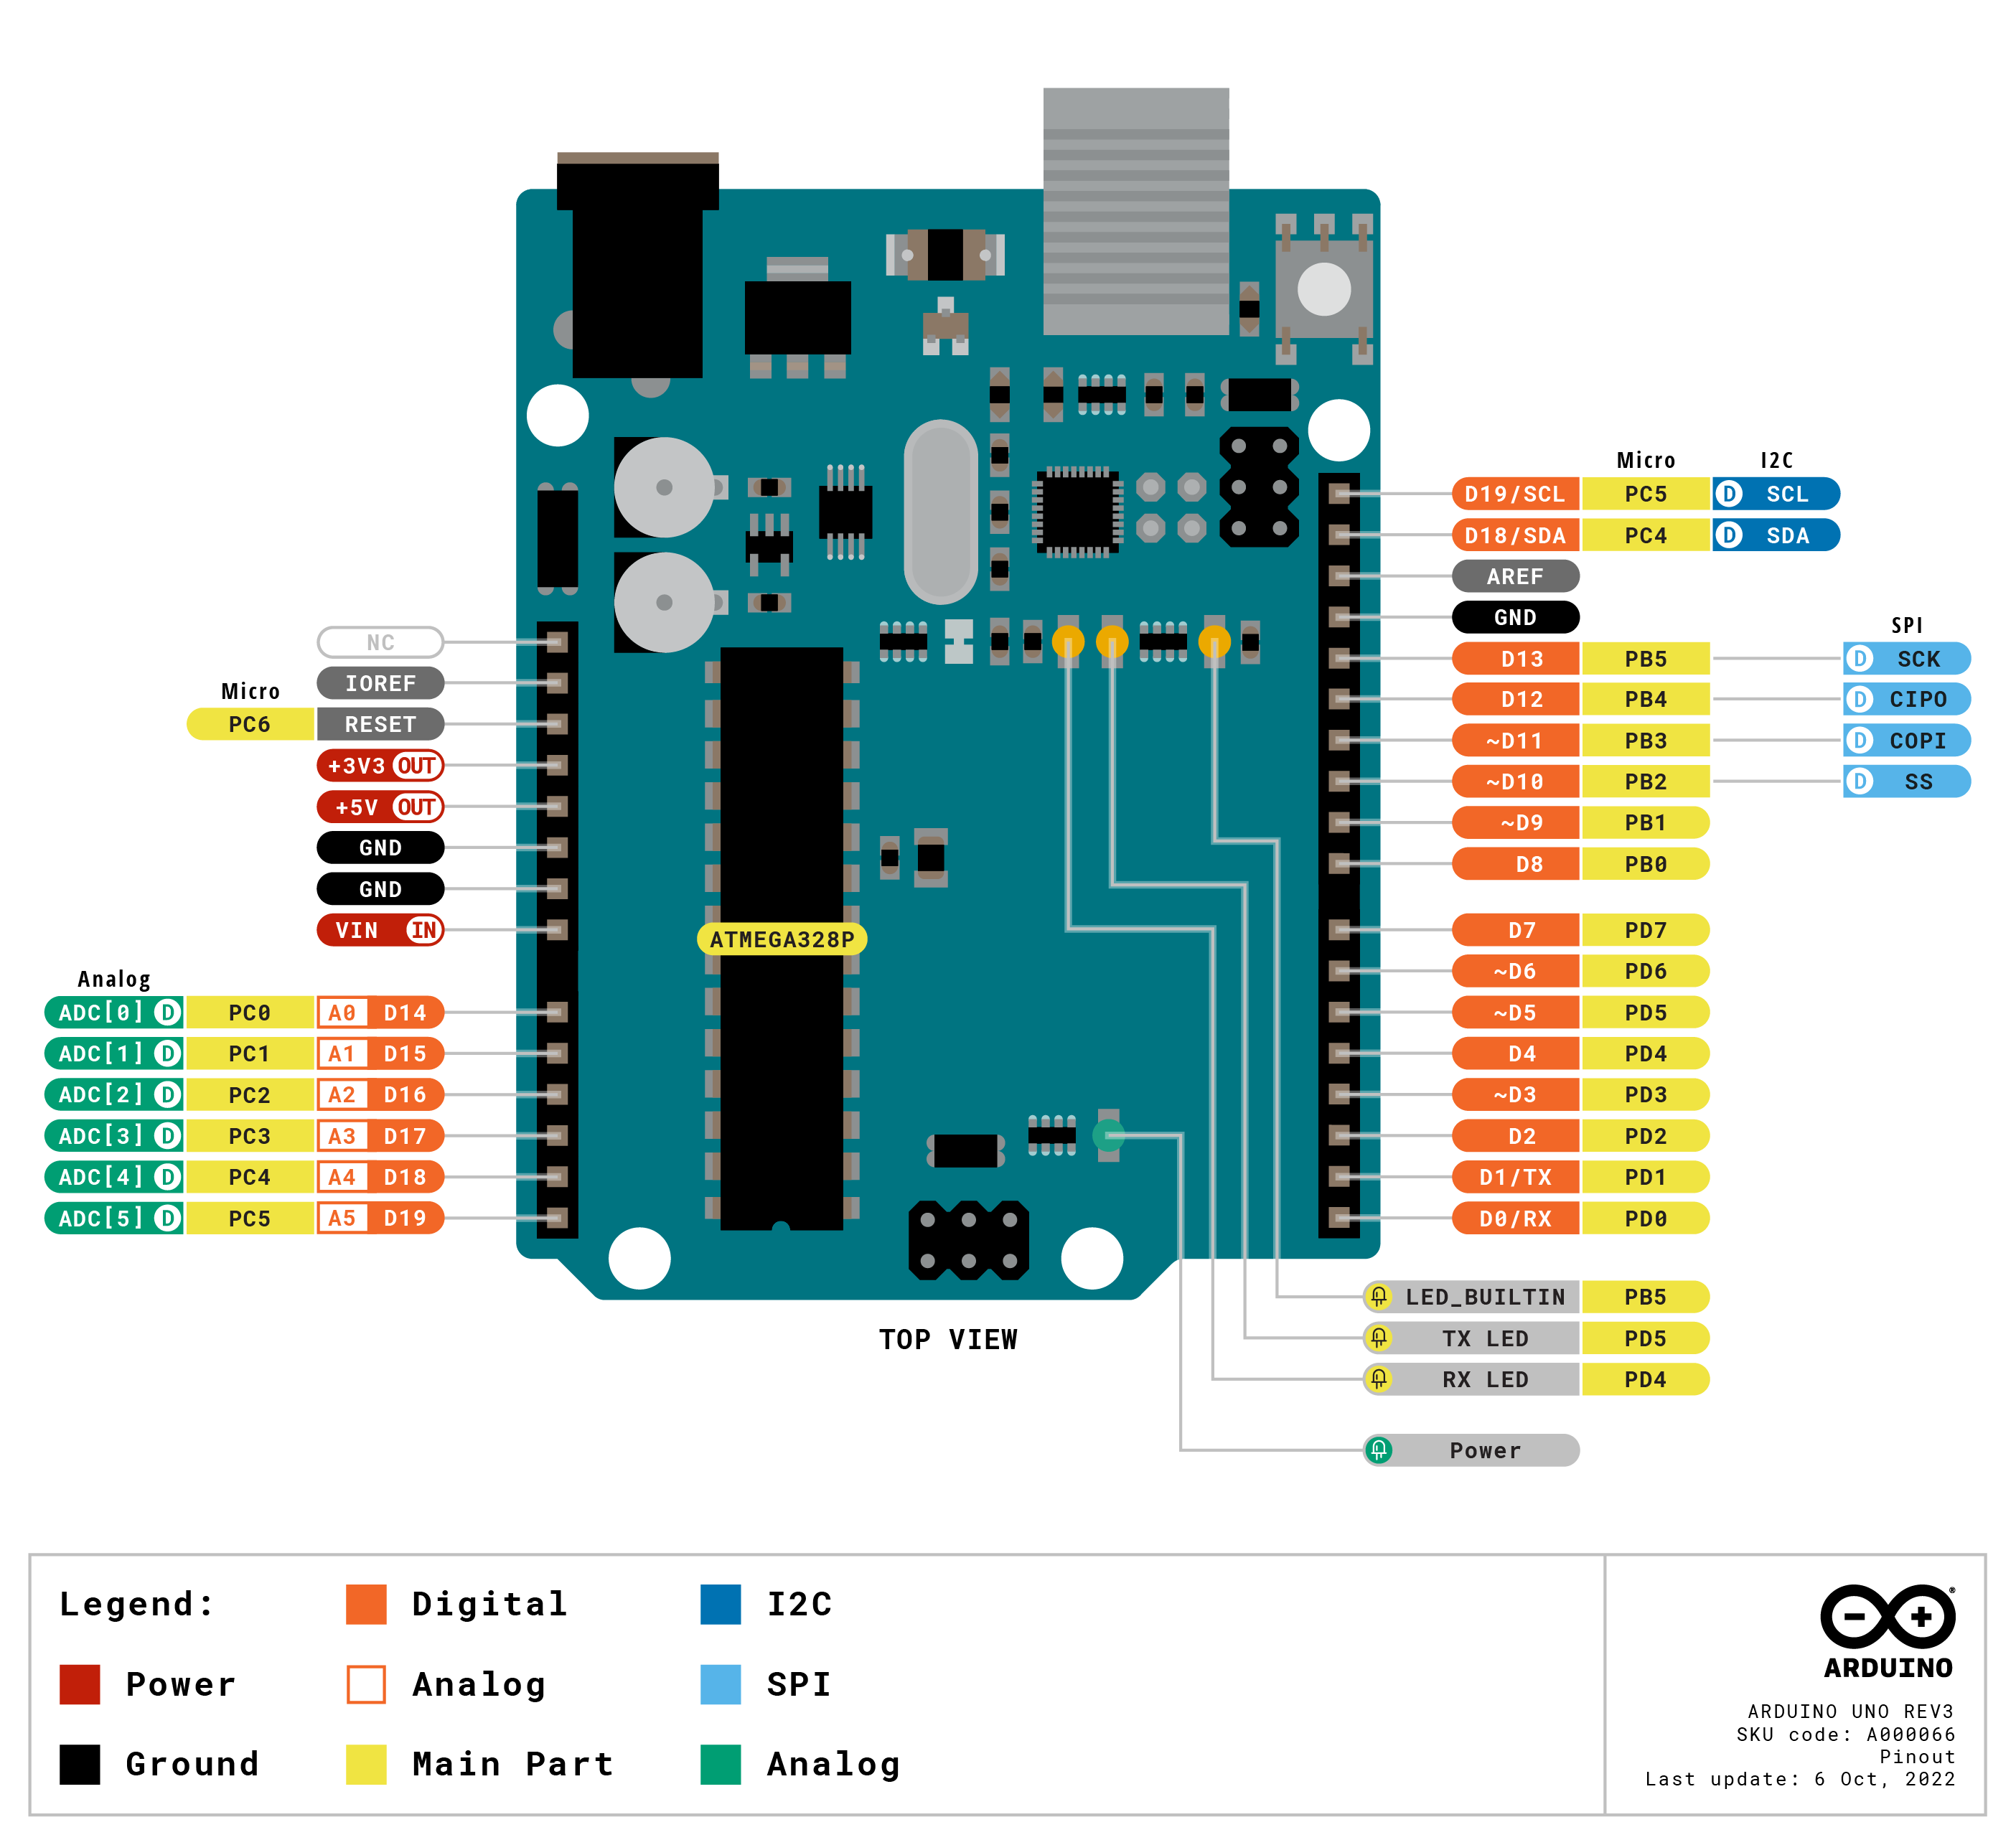
\includegraphics[scale=0.7]{arduino-pinout}
		\caption{Arduino pinout}
		\label{fig:arduino_pinout}
	\end{figure}
	
	
\end{document} 

